In this chapter, 

\section{Architecture}

\begin{figure}[htb]
    \centering
    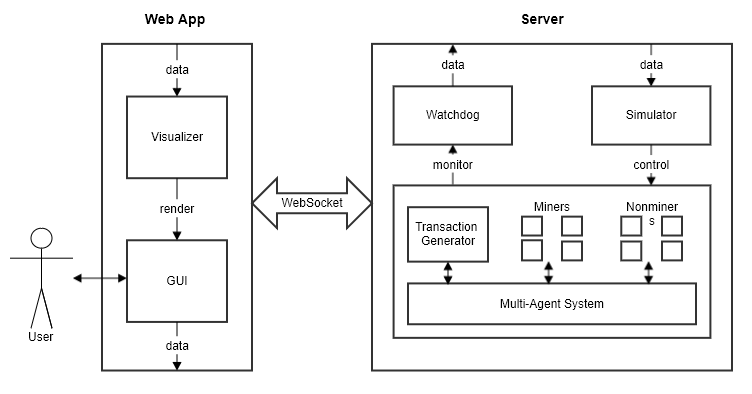
\includegraphics[width=\textwidth]{impl_architecture}
    \caption{Architecture.}
    \label{fig:architecture}
\end{figure}

Figure \ref{fig:architecture} shows the whole architecture of the visualization application. The architecture contains a web app and a server, which are connected with WebSocket. WebSocket technology makes the real-time communications between the web app and the server possible, as the visualization of the real-time mining processes is necessary. The user can interact with the web application through the graphical user interface.

The server maintains the blockchain system. It is composed of three components.

\begin{itemize}
    \item \textbf{Blockchain System} \\
        The blockchain system is based on a multi-agent system. It cointains a transaction generator, multiple miners, and multiple nonminers. The multi-agent system provides communications for these nodes.
    \item \textbf{Simulator} \\
        The simulator is responsible for receiving data from the client side and controlling the blockchain system.
    \item \textbf{Watchdog} \\
        When the blockchain data structures change in the blockchain system, the watchdog will catch these changes, and send them to the web app. 
\end{itemize}

Since the nodes on the blockchain network can be regarded as agents on a multi-agent system, we decided to contruct the blockchain system with a multi-agent system framework. Here, We choose a web-based multi-agent system framework called Eve \cite{eve}. The main features of Eve are stated below.

\begin{itemize}
    \item \textbf{Robustness} \\
        The agents are decoupled and can be maintained independently. Thus, the whole system is still active even an agent fails.
    \item \textbf{Flexibility} \\
        It is flexible to add or remove agents.
    \item \textbf{Reduced complexity} \\
        The complexity of the distributed software design is lower.
    \item \textbf{Scalability} \\
        The limitation of the number of agents does not exist, so the scalability can grow rapidly.
\end{itemize}

In addtion, Eve provides reliable communications with JSON-RPC protocols \cite{jsonrpc}. Therefore, agents can send and understand the JSON format data between each other, and they can be maintained independently in anywhere, e.g., on the cloud or desktops. Eve is an open source project which is implemented in JavaScript, and it is easy to learn. As a result, Eve allows us to construct a distributed blockchain system without worrying about the technical problems such as asynchronous and locking problems.

The server is built in Node.js with Express framework because of it is based on the same programming language of Eve. During the runtime, a transaction generator, miners, and nonminers can be instantiated and destroyed at any time thanks to the flexibility of Eve.

The web application is responsible for the visualization and the interactions with users. There are two components in the web application.

\begin{itemize}
    \item \textbf{Visualizer} \\
        The visualizer is responsible for rendering the visualization of blockchains when it is notified by the watchdog. It receives the data of transactions and blocks from the server and renders them appropriately on the HTML documents.
    \item \textbf{Graphical User Interface} \\
        The GUI provides an index page and a settings page. The index page is for the visualization part, and the settings page displays all the defined parameters in the blockchain system. More details can be refered to \ref{}.
\end{itemize}

The visualization is based on Three.js, a JavaScript framework for rendering 2D and 3D graphics. Three.js uses WebGL as the renderer, and the updating performance is 60 frame per second. The reason to choose Three.js as the visualization framework is that it is an famous open source project, and the community is active. Moreover, Three.js provides basic shapes, e.g., squares and lines, and handles the updating of frames. Therefore, we can focus on optimize the user experience of the visualization without considering the implementation of WebGL.

\section{Simulator}

The simulator is responsible for controlling the blockchain system and handling all the requests from the client. It is unique in the whole system, so it observes to the singleton pattern. The role of the simulator is like a "door" as it is the only gate to communicate with the blockchain system.

After the blockchain system starts, the simulator initializes the status of the blockchain system, i.e., it instantiates necessary nodes according to the configuration. The waiting list of transactions in the transaction generator and the blockchain data structures of miners and nonminers are initialized by the simulator. 

When the user wants to change the parameters, i.e., mining strategies and delays of networks, or the visualizer needs the information of transaction pools and blockchains, the simulator will interact with the blockchain system by setting the parameters or retrieving the required data. The data are sent through WebSocket in real-time.

The simulator is an important component because it hides the details of the implementation of the blockchain system and provides a unique and robust interface for the requests from the client. As a result, it decouples the relationship between the web application and the blockchain system. The detail of the simulator can be refered to \ref{}.

\section{Watchdog}

The watchdog is responsible for monitoring the behaviors of nodes and notifying the visualizer when the data should be updated. It is unique in the whole system, so it also observes to the singleton pattern.

The watchdog watches three kinds of data in the blockchain system.

\begin{itemize}
    \item blockchain data structures
    \item status of transaction pools
    \item status of mining
\end{itemize}

While a miner receives a transaction or a block, a nonminer receives a block, or a miner is solving the puzzle, the watchdog will notify the visualizer in real-time through WebSocket. Therefore, it is guaranteed that the visualization of the data is synchronized with the blockchain system all the time.

With the help of the watchdog, the activities that happened in the blockchain system is recorded completely. Hence, it ensures the correctness of the visualization application. The detail of the watchdog can be refered to \ref{}.

\section{Visualizer}

The visualizer is responsible for rendering the data that are sent from the watchdog. It is the main part of the visualization application because it shows the elegance of visualization. 

Three items are updated by the visualizer continuously.

\begin{itemize}
    \item status bars for transaction pools
    \item status bars for mining
    \item blockchain data structures
\end{itemize}

The status bars for transaction pools and the status bars for mining are auxiliary tools to help the user understand the events that are acctually happening in mining activities. The status bar for transaction pools becomes longer if the pending transactions are growing and vice versa. The status barsfor mining is usually empty, except that the miner is solving the puzzle. It increases each second when the mining activity continuouses. Unlike the real blockchain networks, the time of solving the puzzles is predictable in our visualization application, and it is defined in the parameter of mining strategies. The main area of the visualization is reserved for the blockchain data structures. Squares represent blocks, and they are chained by lines. Different colors of the squares represent the different sources of the blocks. The growth of the blockchain data structures is dynamic and real-time as the mining activities are in progress.

The visualizer expresses fantastic blockchain visualization that is able to attract the user. In addition, it explains the steps of mining processes understandably, even for the viewers who are new to blockchain technology. The detail of the visualizer can be refered to \ref{}.

\section{UML Diagram}

\begin{figure}[htb]
    \centering
    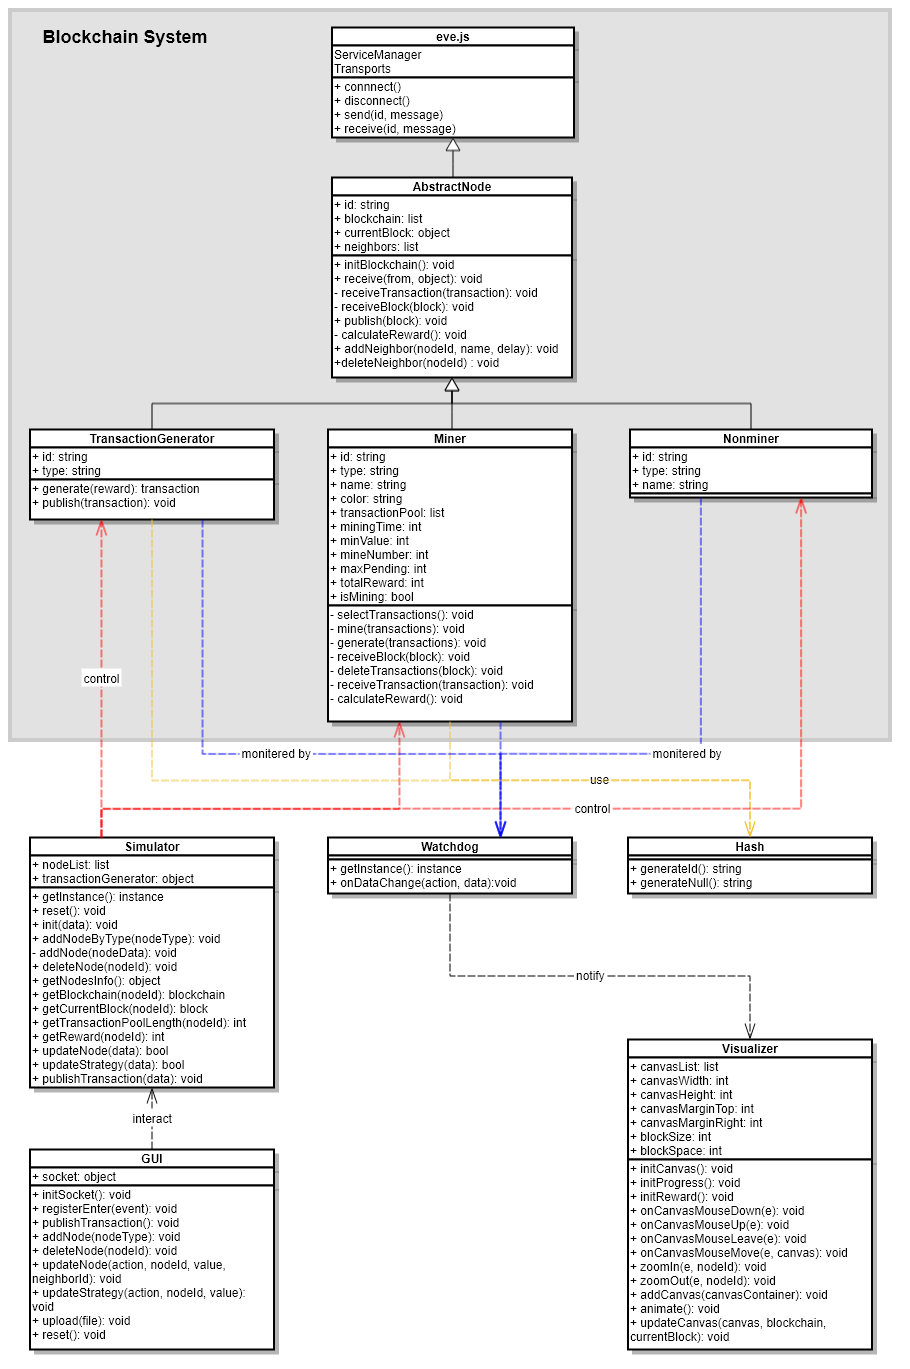
\includegraphics[width=\textwidth]{impl_uml}
    \caption{Class Diagram.}
    \label{fig:class diagram}
\end{figure}

In Figure \ref{fig:class diagram}, it demonstrates the class diagram of the visualization application. The blockchain system is based on the multi-agent system framework Eve. Abstract class \texttt{AbstractNode} defines the common properties and methods of class \texttt{TransactionGenerator}, class \texttt{Miner}, and class \texttt{Nonminer}, and because it is abstract, it is not allowed to instantiate from \texttt{AbstractNode}. In contrast, we can instantiate objects from the children of \texttt{AbstractNode}, i.e., \texttt{TransactionGenerator}, \texttt{Miner}, and \texttt{Nonminer}.

\section{Algorithms}
\label{algorithms}

The mining algorithm determines the most important part of the blockchain system. Miners generate blocks by following the logic of the mining algorithm, but with different parameters that are defined in their own mining strategies. To start mining a block, miners must select a set of pending transactions from their own transaction pools. There are two cases when selecting transactions. If the transaction pool contains too much number of transactions, then the miner ignores the parameter of the minimum value of transactions and selects a set of transactions with the highest values. On the other hand, the miner selects a set of transactions which values are higher than the minimum value of transactions. After the selection of transactions, if the number of selected transactions satisfies the number of transactions that should be included in a block, then the miner will start mining.

Another important algorithm is about the consensus protocol. The algorithm of the consensus protocol is very simple because we do not consider malicious nodes in the blockchain system currently. Therefore, it is only responsible for resolving the longest blockchain. When a node receives a block from other nodes, this algorithm is triggered. If the received block is at a higher layer, i.e., the blockchain becomes longer, then the node will switch the current block to the received block to ensures that it is working on the correct blockchain. Moreover, the transactions of the received block are deleted from the transaction pools because these transactions are not pending anymore.

\section{Configuration Files}

To replay the same visualization of blockchain processes, we can define the configuration of the blockchain system in a file and upload it to the application. The configuration file is composed of three parts: the properties and the parameters of mining strategies of nodes, the delays of networks between each node, and the transactions that will be published through the network. The file is in JSON format, and the file is uploaded to initialize the blockchain system at the beginning.

First, for nodes, it is important to define a unique transaction generator at first, and then it is followed by miners and nonminers. After that, a list of delays between each node is defined. As mentioned before, the transaction generator only connects to miners, and miners and nonminers connect with each other. In the last part, it contains a list of transactions with rewards and the time when the transaction will be published after the starting of the blockchain system.
